\begin{pastexam}[label={px:gw3-106-ds-01}]{關務三等資訊處理 106 年 第一題}
（申論；25 分）

一個二元搜尋樹（binary search tree）初始為空的，依序插入（insert）5,11,9,24,10,2,15,3。
\begin{enumerate}[leftmargin=2.6em, labelsep=0.4em]
\item[㈠] 請繪出完成輸入後的二元搜尋樹。（10 分）
\item[㈡] 試說明如何利用一維陣列來表示（represent）此二元搜尋樹，並在此一維陣列中保有此樹狀結構父節點與子節點的
關係性。（5 分）
\item[㈢] 請設計一演算法能將此二元搜尋樹，依數值由大到小的方式輸出。（5 分）
\item[㈣] 對㈠產生的二元搜尋樹，刪除數值 5。請繪出完成刪除動作後的二元搜尋樹。（5 分）
\end{enumerate}
\end{pastexam}

\begin{pastsoln}
\textbf{㈠} 逐一插入（資結書第~9.2~節，小往左、大往右）：5 當根；$11 > 5$ 放 5 的右子；9：$> 5$、$< 11$，放 11 的
左子；24：$> 5$、$> 11$，放 11 的右子；10：$> 5$、$< 11$、$> 9$，放 9 的右子；2：$< 5$，放 5 的左子；
15：$> 5$、$> 11$、$< 24$，放 24 的左子；3：$< 5$、$> 2$，放 2 的右子。
\begin{center}
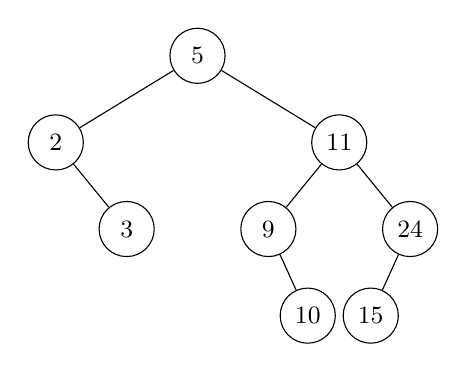
\begin{tikzpicture}[n/.style={circle,draw,inner sep=0pt,minimum size=7mm,font=\small},
  level distance=11mm, level 1/.style={sibling distance=36mm}, level 2/.style={sibling distance=18mm},
  level 3/.style={sibling distance=10mm}]
\node[n] {5}
  child {node[n] {2} child[missing] child {node[n] {3}}}
  child {node[n] {11}
    child {node[n] {9} child[missing] child {node[n] {10}}}
    child {node[n] {24} child {node[n] {15}} child[missing]}};
\end{tikzpicture}
\end{center}
中序走訪 $2, 3, 5, 9, 10, 11, 15, 24$ 由小到大，樹是對的。

\textbf{㈡} 用資結書第~7.2.1~節的陣列表示法：把樹想成補滿的完整二元樹，由上到下、由左到右編號，根是 $1$；
節點 $i$ 的左子在 $2i$、右子在 $2i + 1$、父節點在 $\lfloor i/2 \rfloor$，不存在的節點那一格留空（或放一個特殊值）。
這棵樹：根 5 在 $1$；2、11 在 $2$、$3$；2 的右子 3 在 $5$；11 的子 9、24 在 $6$、$7$；9 的右子 10 在 $13$；24 的
左子 15 在 $14$。
\begin{center}
\small
\setlength{\tabcolsep}{4pt}
\begin{tabular}{c|cccccccccccccc}
下標 & 1 & 2 & 3 & 4 & 5 & 6 & 7 & 8 & 9 & 10 & 11 & 12 & 13 & 14 \\
\hline
值 & 5 & 2 & 11 & -- & 3 & 9 & 24 & -- & -- & -- & -- & -- & 10 & 15 \\
\end{tabular}
\end{center}
父子關係完全由下標算出，例如 $A[6] = 9$ 的右子是 $A[13] = 10$，$A[14] = 15$ 的父節點是 $A[7] = 24$。 缺點：樹不完整
時會有空格，這棵 $8$ 個節點的樹用了 $14$ 格；高度 $h$ 的樹最多要 $2^h - 1$ 格，退化成一條鏈時非常浪費。

另一種不浪費空間的陣列表示法是每格存（值，左子下標，右子下標），用下標代替指標：
依插入順序編號，$1{:}(5, 6, 2)$、$2{:}(11, 3, 4)$、$3{:}(9, 0, 5)$、$4{:}(24, 7, 0)$、$5{:}(10, 0, 0)$、$6{:}(2, 0, 8)$、
$7{:}(15, 0, 0)$、$8{:}(3, 0, 0)$，其中 $0$ 表示沒有子節點，只用 $8$ 格。 需要往上走時，再加一欄父節點下標。

\textbf{㈢} 中序走訪（左、根、右）輸出由小到大；把左右對調，用「右、根、左」的反向中序走訪，就是由大到小：
\begin{pseudo}{由大到小輸出二元搜尋樹}
\Procedure{Reverse-Inorder}{$x$}
    \If{$x \ne \NIL$}
        \State \Call{Reverse-Inorder}{$x.\mathit{right}$} \Comment{比 $x$ 大的先輸出}
        \State 輸出 $x.\mathit{key}$
        \State \Call{Reverse-Inorder}{$x.\mathit{left}$} \Comment{再輸出比 $x$ 小的}
    \EndIf
\EndProcedure
\end{pseudo}
正確性：對子樹大小歸納，右子樹的鍵都比 $x$ 大、左子樹的都比 $x$ 小，各自由大到小輸出，接起來就是整棵由大到小。
每個節點處理一次，時間 $\Theta(n)$。 這棵樹輸出 $24, 15, 11, 10, 9, 5, 3, 2$。

\textbf{㈣} 5 是根，有兩個子節點，用中序後繼頂替（資結書虛擬碼~9.7）：右子樹（根 11）一路往左，$11 \to 9$，9 沒有
左子，後繼是 9。 9 有右子 10，先把 9 從原位置移走、由 10 接到 11 的左邊，再把根的值換成 9：
\begin{center}
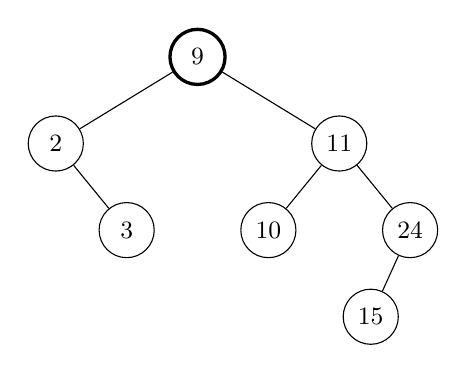
\begin{tikzpicture}[n/.style={circle,draw,inner sep=0pt,minimum size=7mm,font=\small},
  level distance=11mm, level 1/.style={sibling distance=36mm}, level 2/.style={sibling distance=18mm},
  level 3/.style={sibling distance=10mm}]
\node[n,very thick] {9}
  child {node[n] {2} child[missing] child {node[n] {3}}}
  child {node[n] {11}
    child {node[n] {10}}
    child {node[n] {24} child {node[n] {15}} child[missing]}};
\end{tikzpicture}
\end{center}
中序 $2, 3, 9, 10, 11, 15, 24$，正是原序列去掉 5。 改用中序前驅（左子樹最大的 3）頂替也可以：根變成 3，2 的右子
變成空，右子樹不變。
\end{pastsoln}
